\documentclass{beamer} % [aspectratio=169]
 
\usepackage[utf8]{inputenc}
\usepackage[danish]{babel}
\usepackage{natbib}
\usepackage{graphicx}
\usepackage{amsmath}
\usepackage{amsfonts}
\usepackage{amssymb}
\usepackage{amsthm}
\usepackage{tikz}
\newcommand{\R}{\mathbb{R}}
\newcommand{\CC}{\mathbb{C}}
\newcommand{\F}{\mathbb{F}}
\newcommand{\K}{\mathbb{K}}

\newcommand{\borel}{\mathcal{B}}
\newcommand{\sE}{\mathcal{E}}

\newcommand{\isomorph}{\cong}

\newcommand{\fat}[1]{\mathbf{#1}}
\newcommand{\curly}[1]{\{#1\}}
\newcommand{\para}[1]{\left(#1\right)}
\newcommand{\makeset}[2]{\curly{#1 \mid #2}}
\newcommand{\makesetcolon}[2]{\curly{#1 \, : \, #2}}
\newcommand{\openint}[2]{\mathopen]#1, #2\mathclose[}
\newcommand{\closedint}[2]{\mathopen[#1, #2\mathclose]}
\newcommand{\fracp}[2]{\left(\frac{#1}{#2}\right)}
\newcommand{\abs}[1]{\left\lvert #1 \right\rvert}
\newcommand{\norm}[1]{\left\lVert #1 \right\rVert}
\newcommand{\ip}[2]{\langle #1, #2\rangle}
\newcommand{\generator}[1]{\langle#1\rangle}
\newcommand{\paraip}[2]{\left\langle #1, #2\right\rangle}
\newcommand{\comment}[1]{\quad \para{\text{#1}}}

\newcommand{\longpause}{\break \break \pause}

% CompGeo
\DeclareMathOperator{\dist}{dist}
\DeclareMathOperator{\Vor}{Vor}
\DeclareMathOperator{\VorG}{Vor_{G}}
\DeclareMathOperator{\bi}{bi}

\usetheme{Madrid}

\title{Specialeforsvar}
\author{Johannes Jensen}
\institute{Aarhus Universitet}
\date{\today}
 
\begin{document}
 
\frame{\titlepage}

\begin{frame}
\pause
\[
	\huge\text{Introduktion}
\]
\end{frame}

\begin{frame}
\pause
\[
	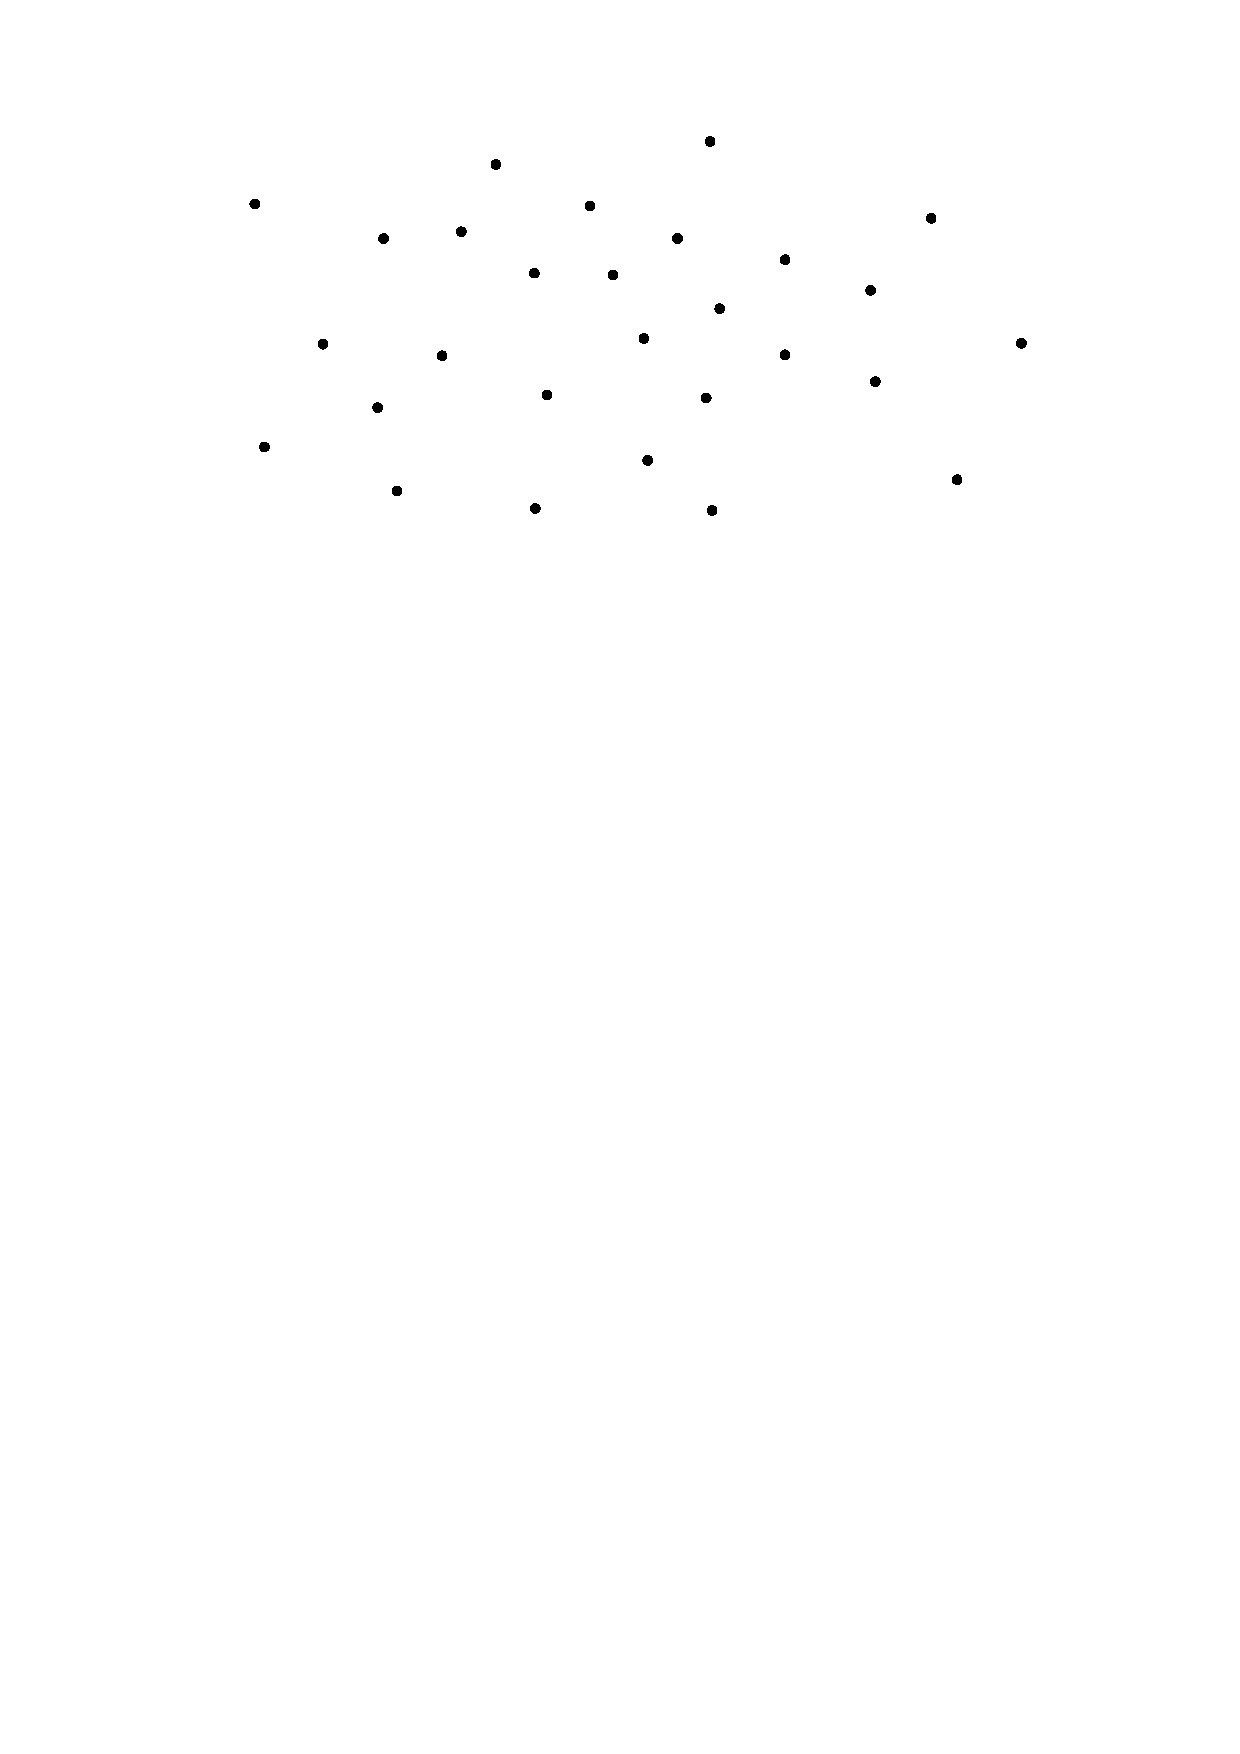
\includegraphics[scale=0.7]{images/intro_without_diagram}
\]
Lad $P = \curly{p_1, p_2, \ldots, p_n} \subset \R^2$ betegne en endelig mængde af \textit{sites}.
\end{frame}

\begin{frame}
\[
	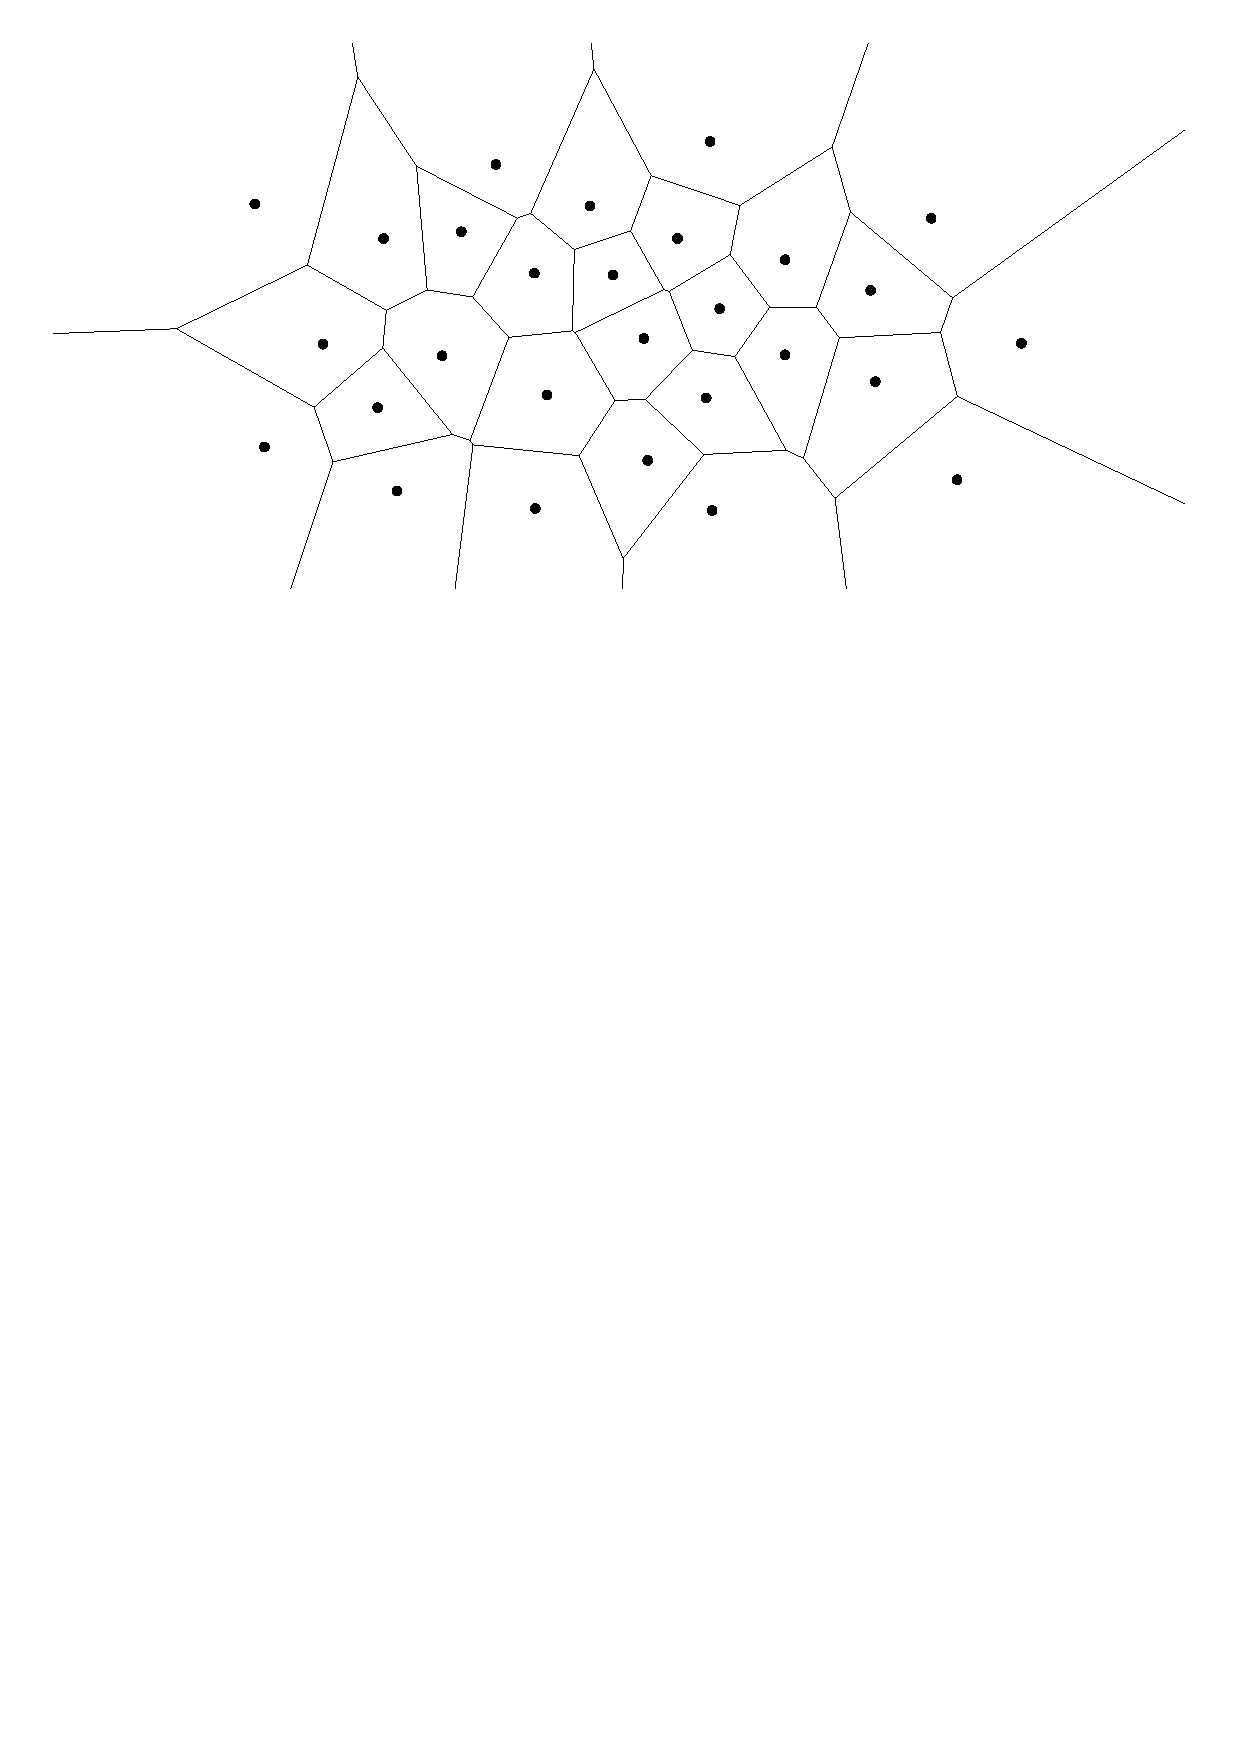
\includegraphics[scale=0.7]{images/intro_with_diagram}
\]
Vi ønsker så at beregne $\Vor(P)$, \textit{Voronoi diagrammet} for $P$.
\end{frame}

\begin{frame}
\[
	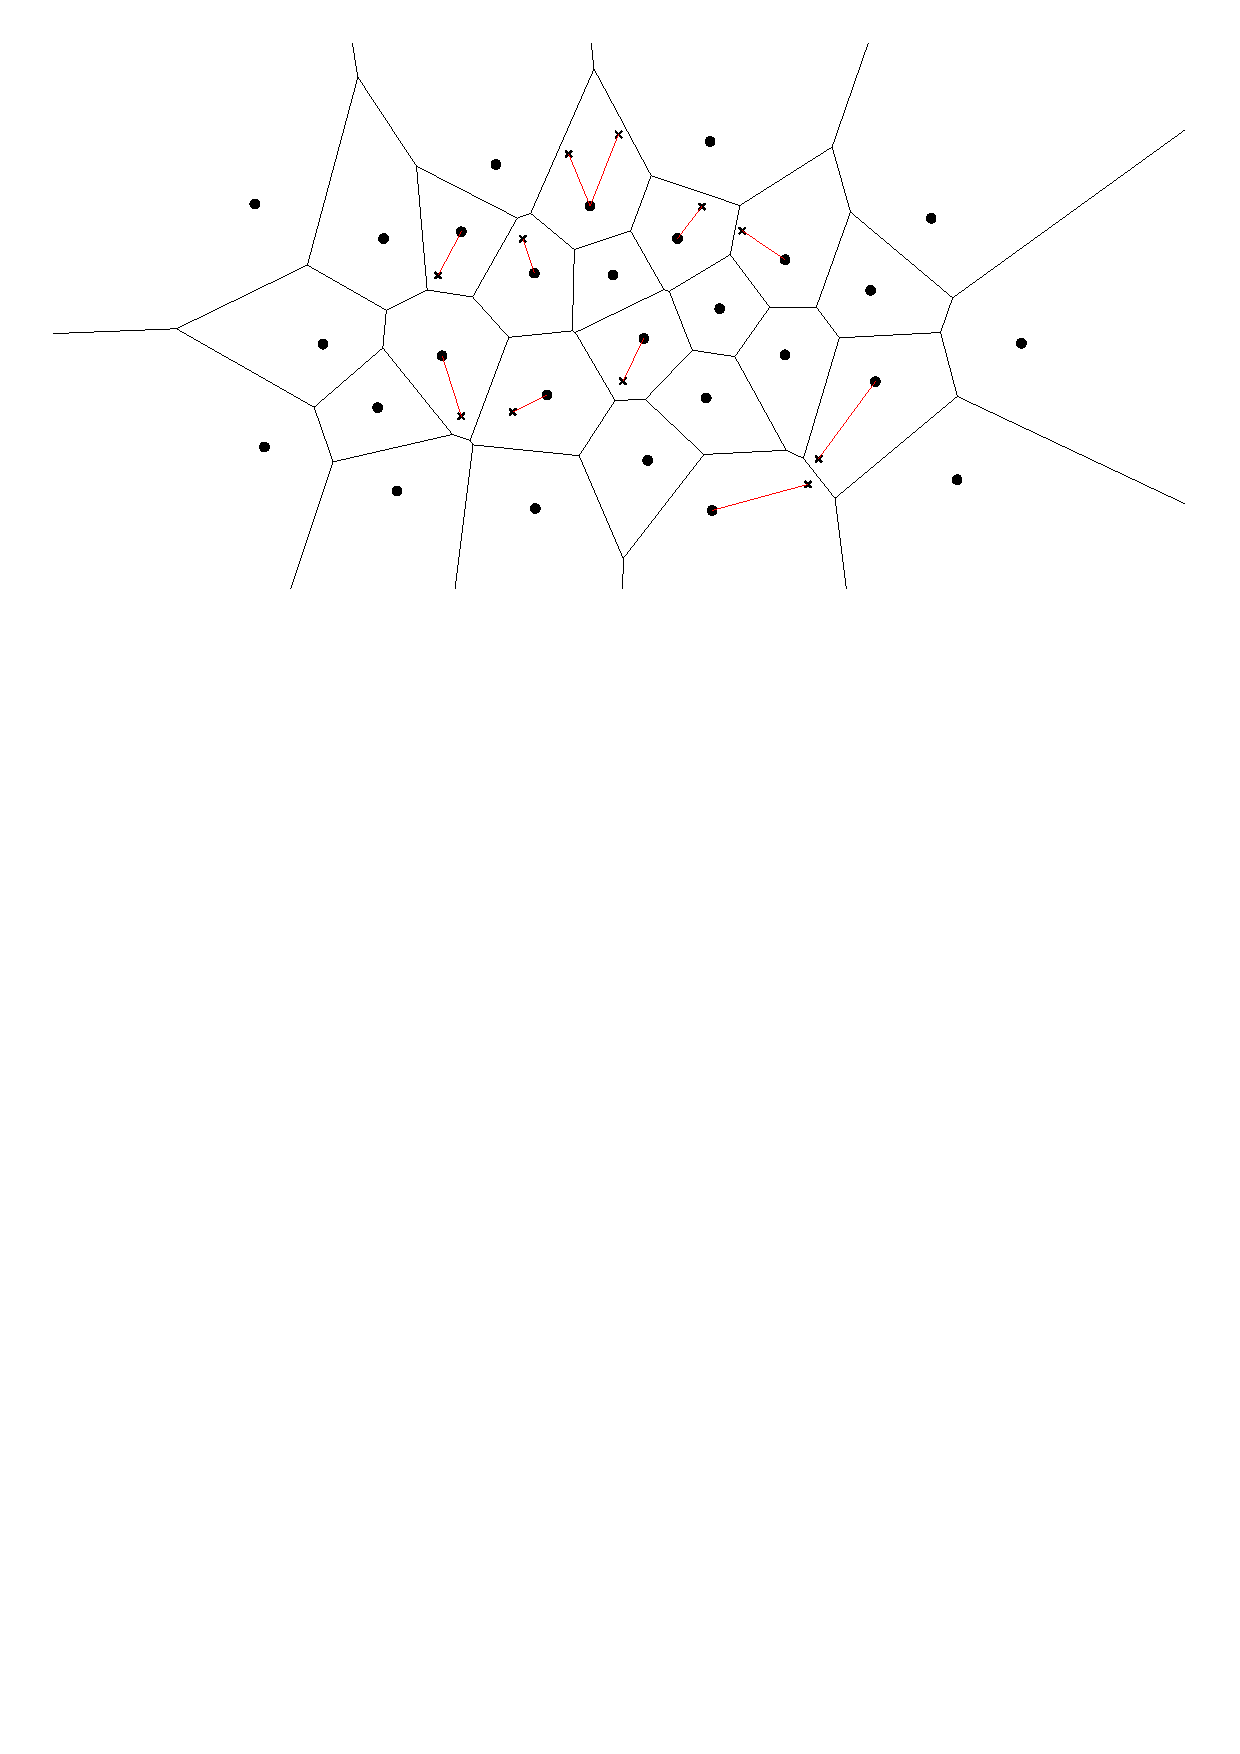
\includegraphics[scale=0.7]{images/intro_distances}
\]
Hvad kan Voronoi diagrammet? Givet et $\times$ i en \textit{Voronoi celle} angiver diagrammet hvilket punkt fra $P$ som er tættest på!
\end{frame}

\begin{frame}
\pause
Men hvordan beregner man det?
\longpause
Man bruger en \textit{sweep line algorithm}! (En fejende linje algoritme...?)
\longpause
Demo tid!
\end{frame}

\begin{frame}
\pause
Hvorfor virker det?
\longpause
\[
	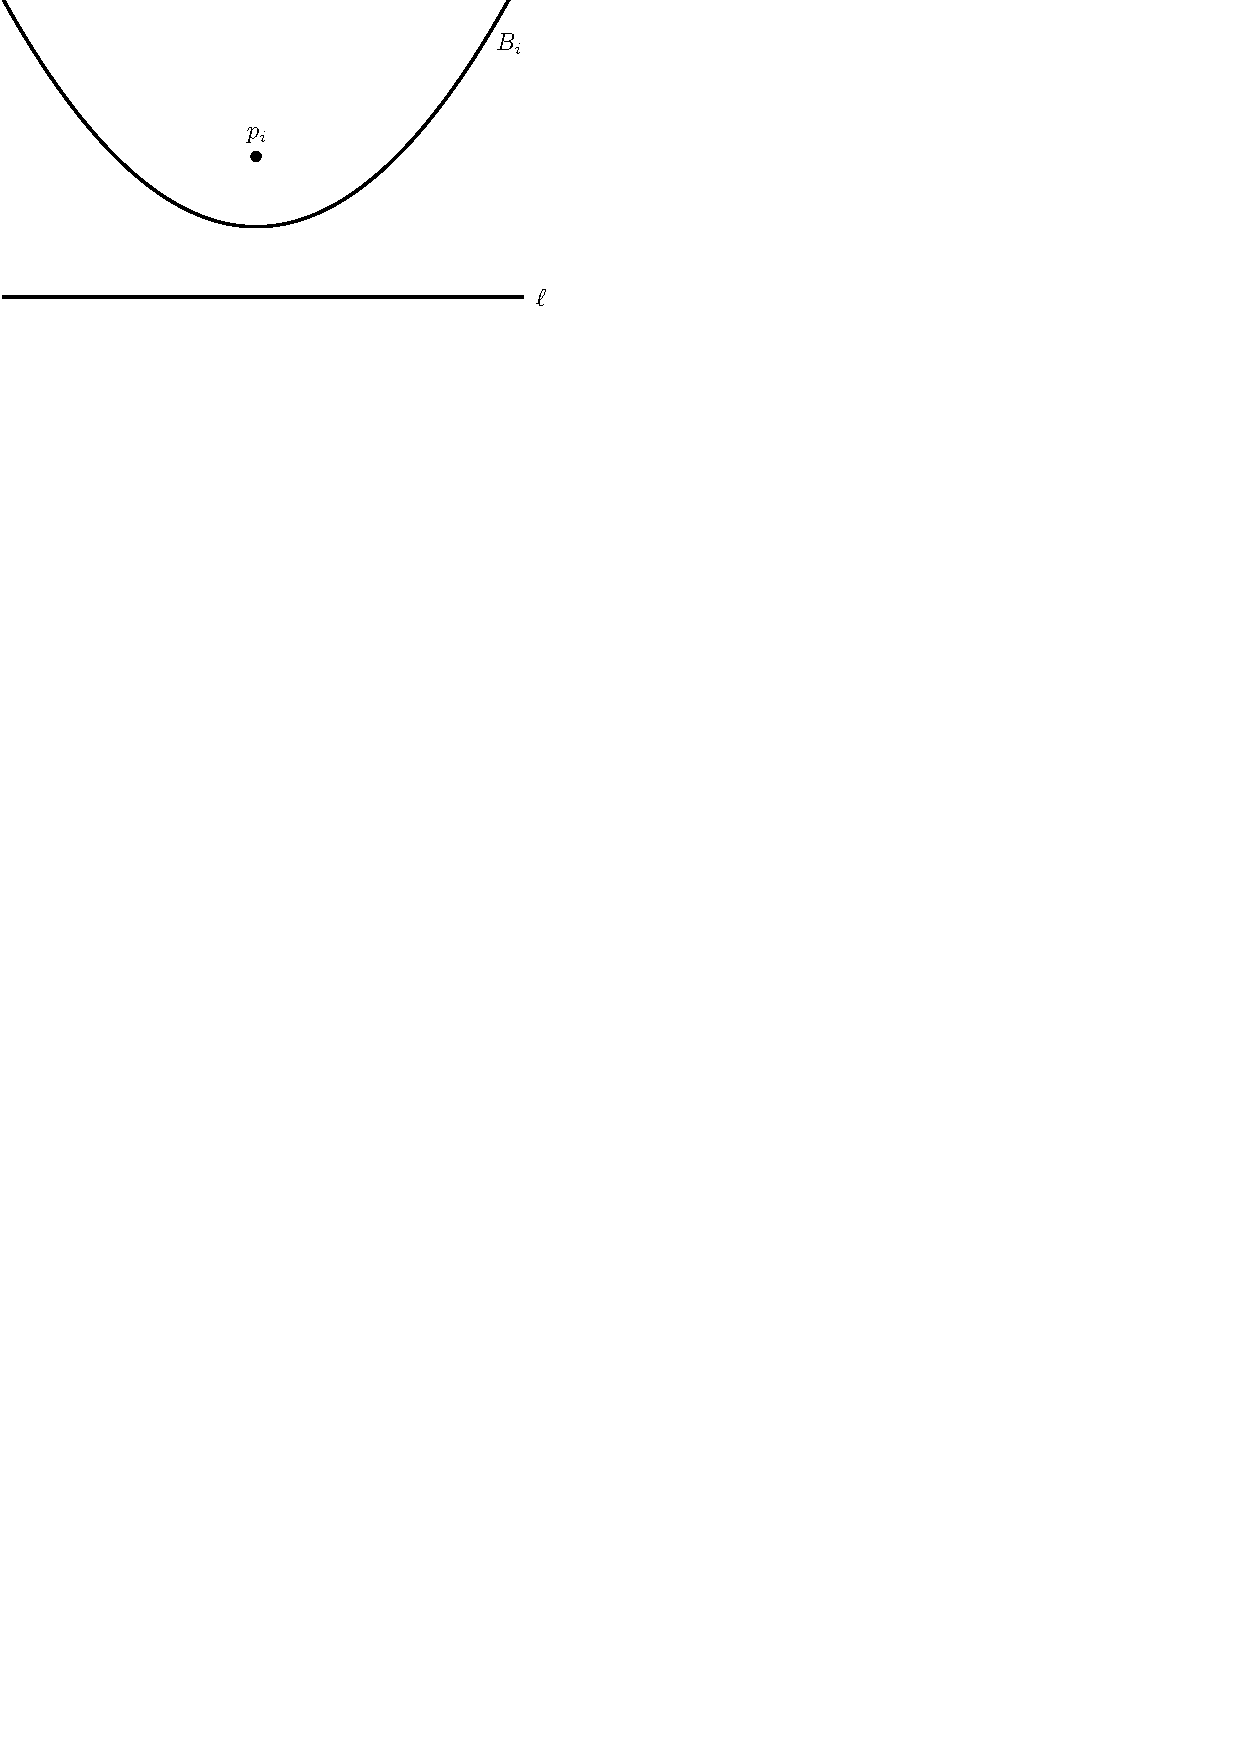
\includegraphics[scale=0.9]{../images/hyperbola_intro}
\]
Vi kan separere ethvert site $p_i \in P$ og vores sweep line $\ell$ med en andengrads kurve $B_i$\pause, således at for alle $q \in B_i$ så $\dist(q, p_i) = \dist(q, \ell)$.
\end{frame}

\begin{frame}
\pause
Vi kan så gøre dette for alle sites i $P$, men vi beholder kun de dele af kurverne som ligger tættest på $\ell$:
\[
	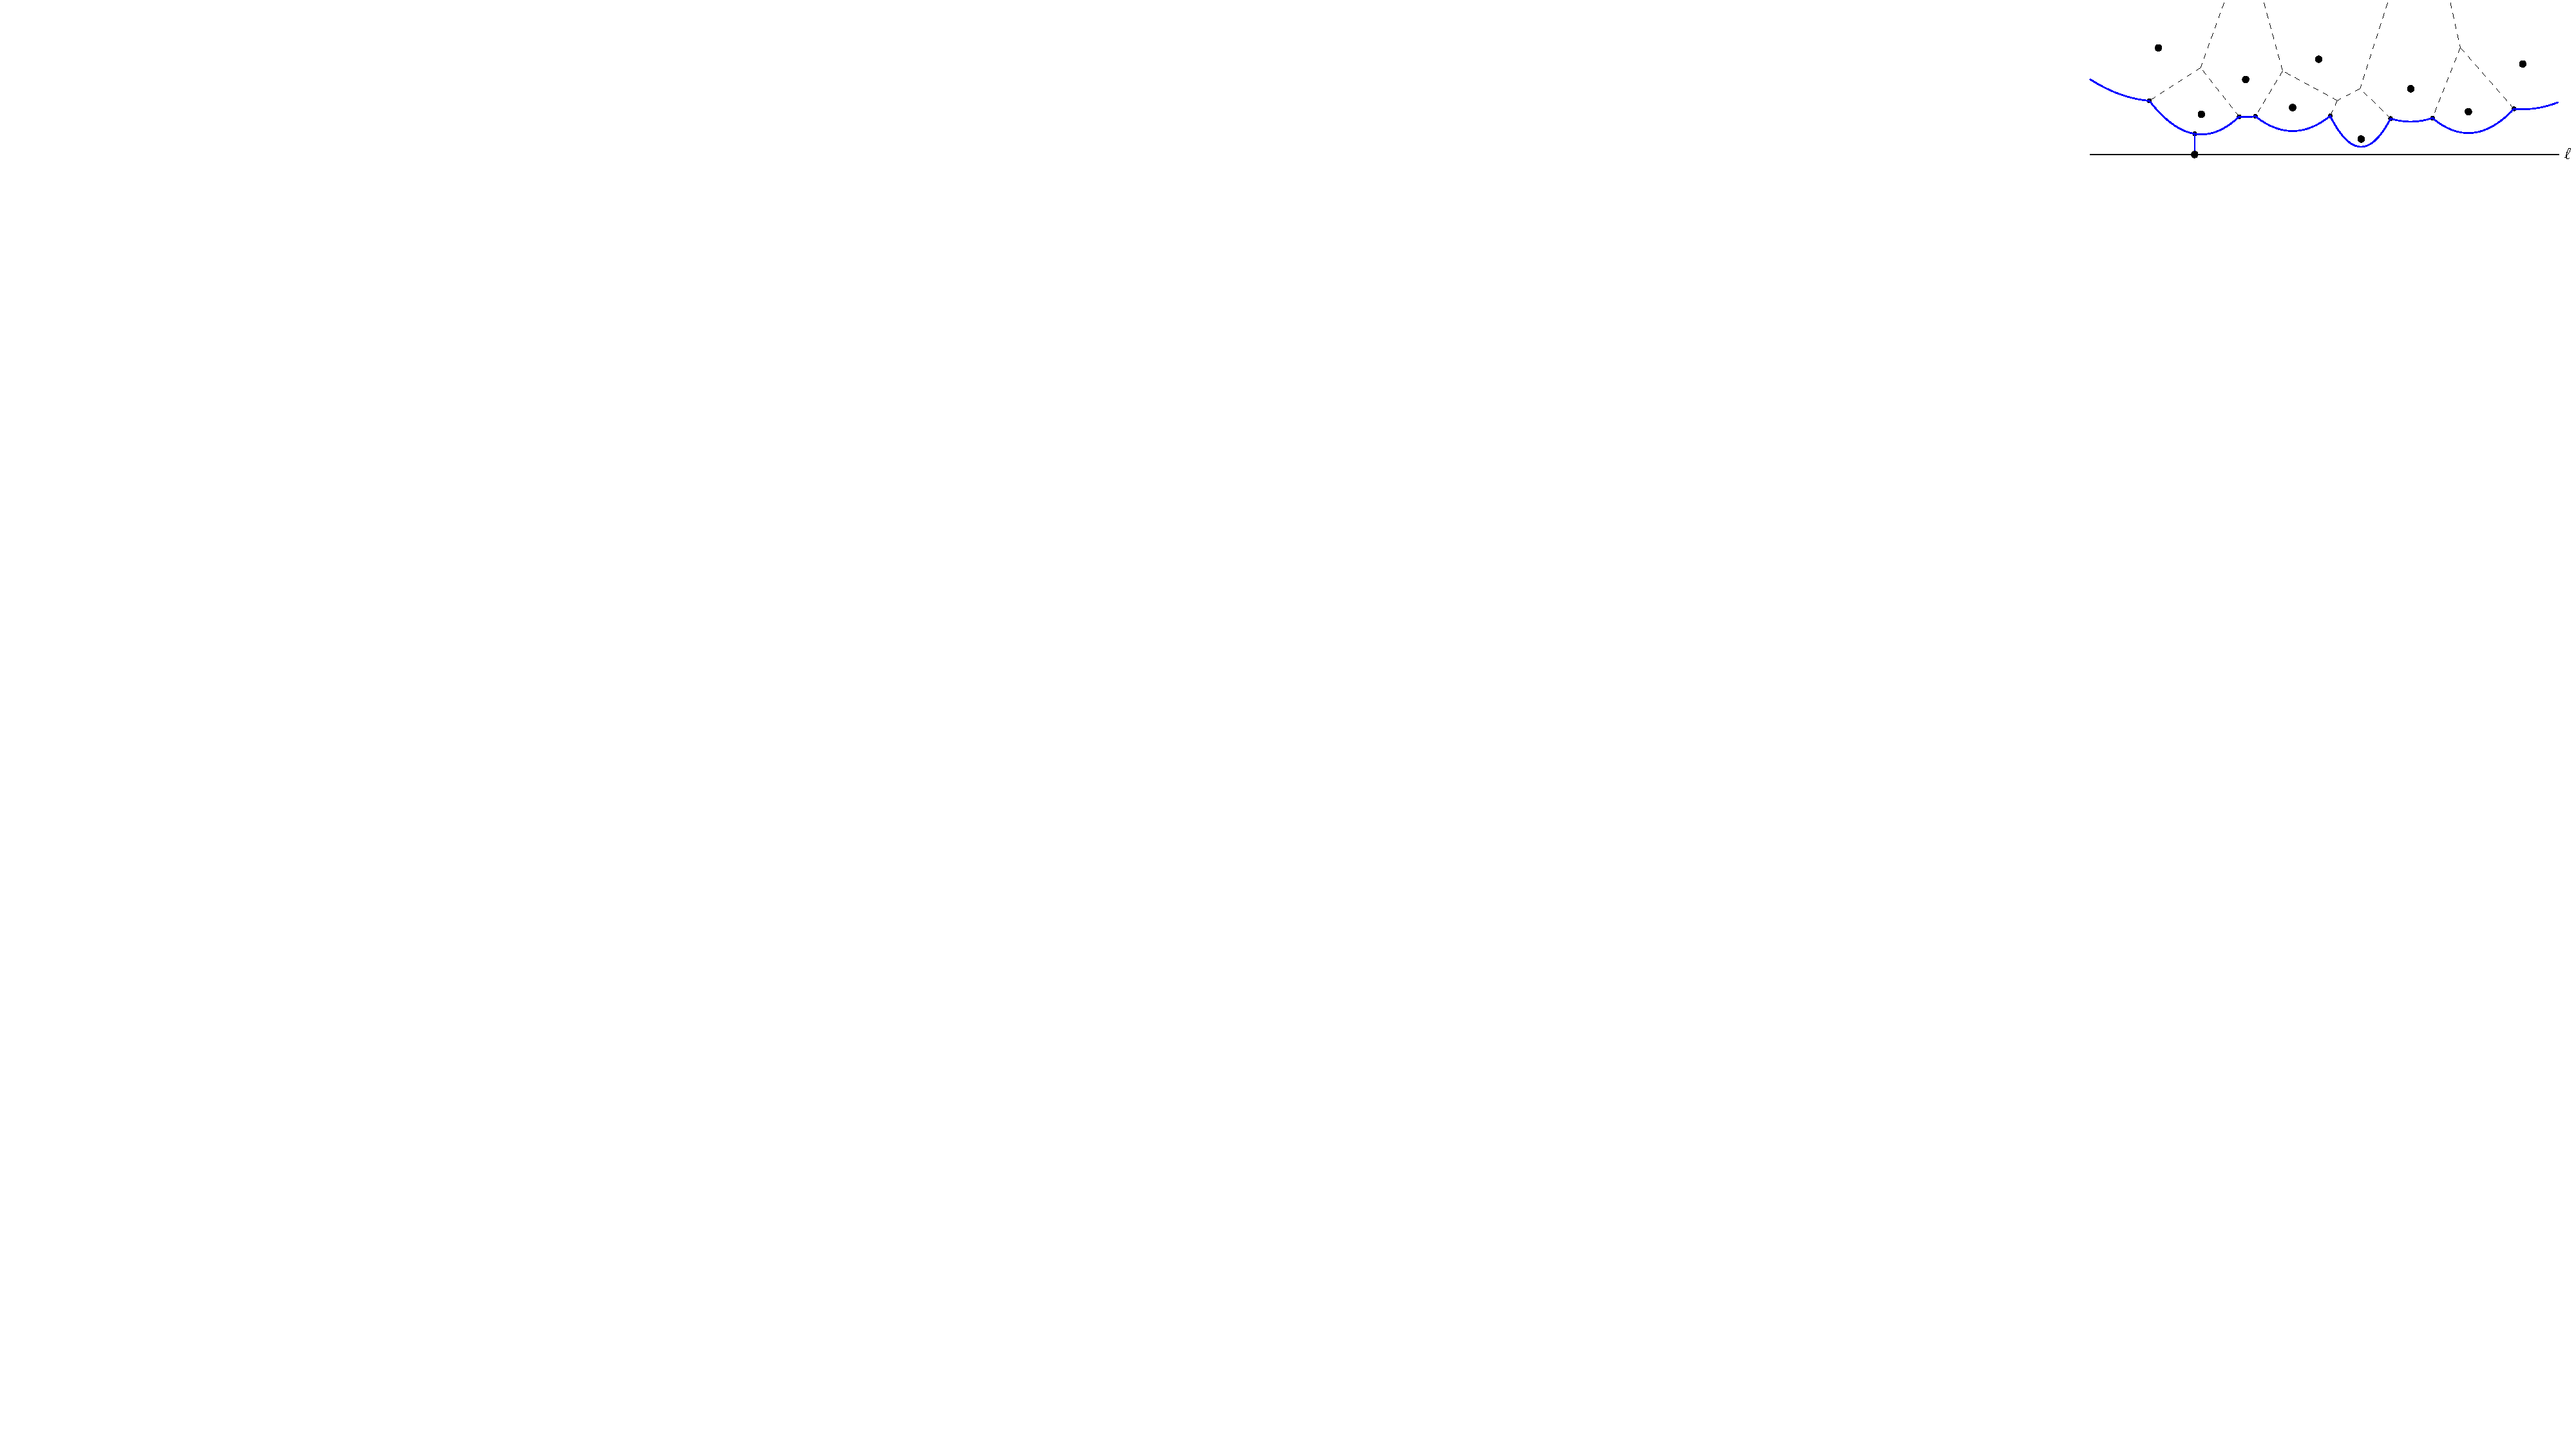
\includegraphics[scale=0.8]{../images/beachline}
\]
\pause
Den blå kurve kalder vi for \textit{the beach line} (kystlinjen) for $\ell$ mht. $P$.
\longpause
At sweep line metoden virker følger så fra at skæringerne mellem forskellige $B_i$ og $B_j$ \pause optegner Voronoi diagrammet når vi fejer $\ell$ fra ``$y = \infty$'' til ``$y = -\infty$''.
\end{frame}

\begin{frame}
\pause
Men hvordan får man en computer til at gå igennem alle mulige positioner for $\ell$, der er jo uendeligt mange af dem?
\longpause
Nøgleindsigt: Vi behøver kun at holde øje med de positioner for $\ell$ hvor kystlinjens topologiske struktur ændrer sig!
\longpause
Vi vil finde de positioner for $\ell$ hvor der bliver \textit{tilføjet} en kurve til kystlinjen\pause, og de tidspunkter hvor der bliver \textit{fjernet} en kurve fra kystlinjen.
\longpause
Dette kan illustreres med blot 3 punkter (Demo tid!)
\end{frame}

\begin{frame}
\pause
Vi så at der bliver tilføjet en kurve til kystlinjen når $\ell$ rammer en site.
\[
	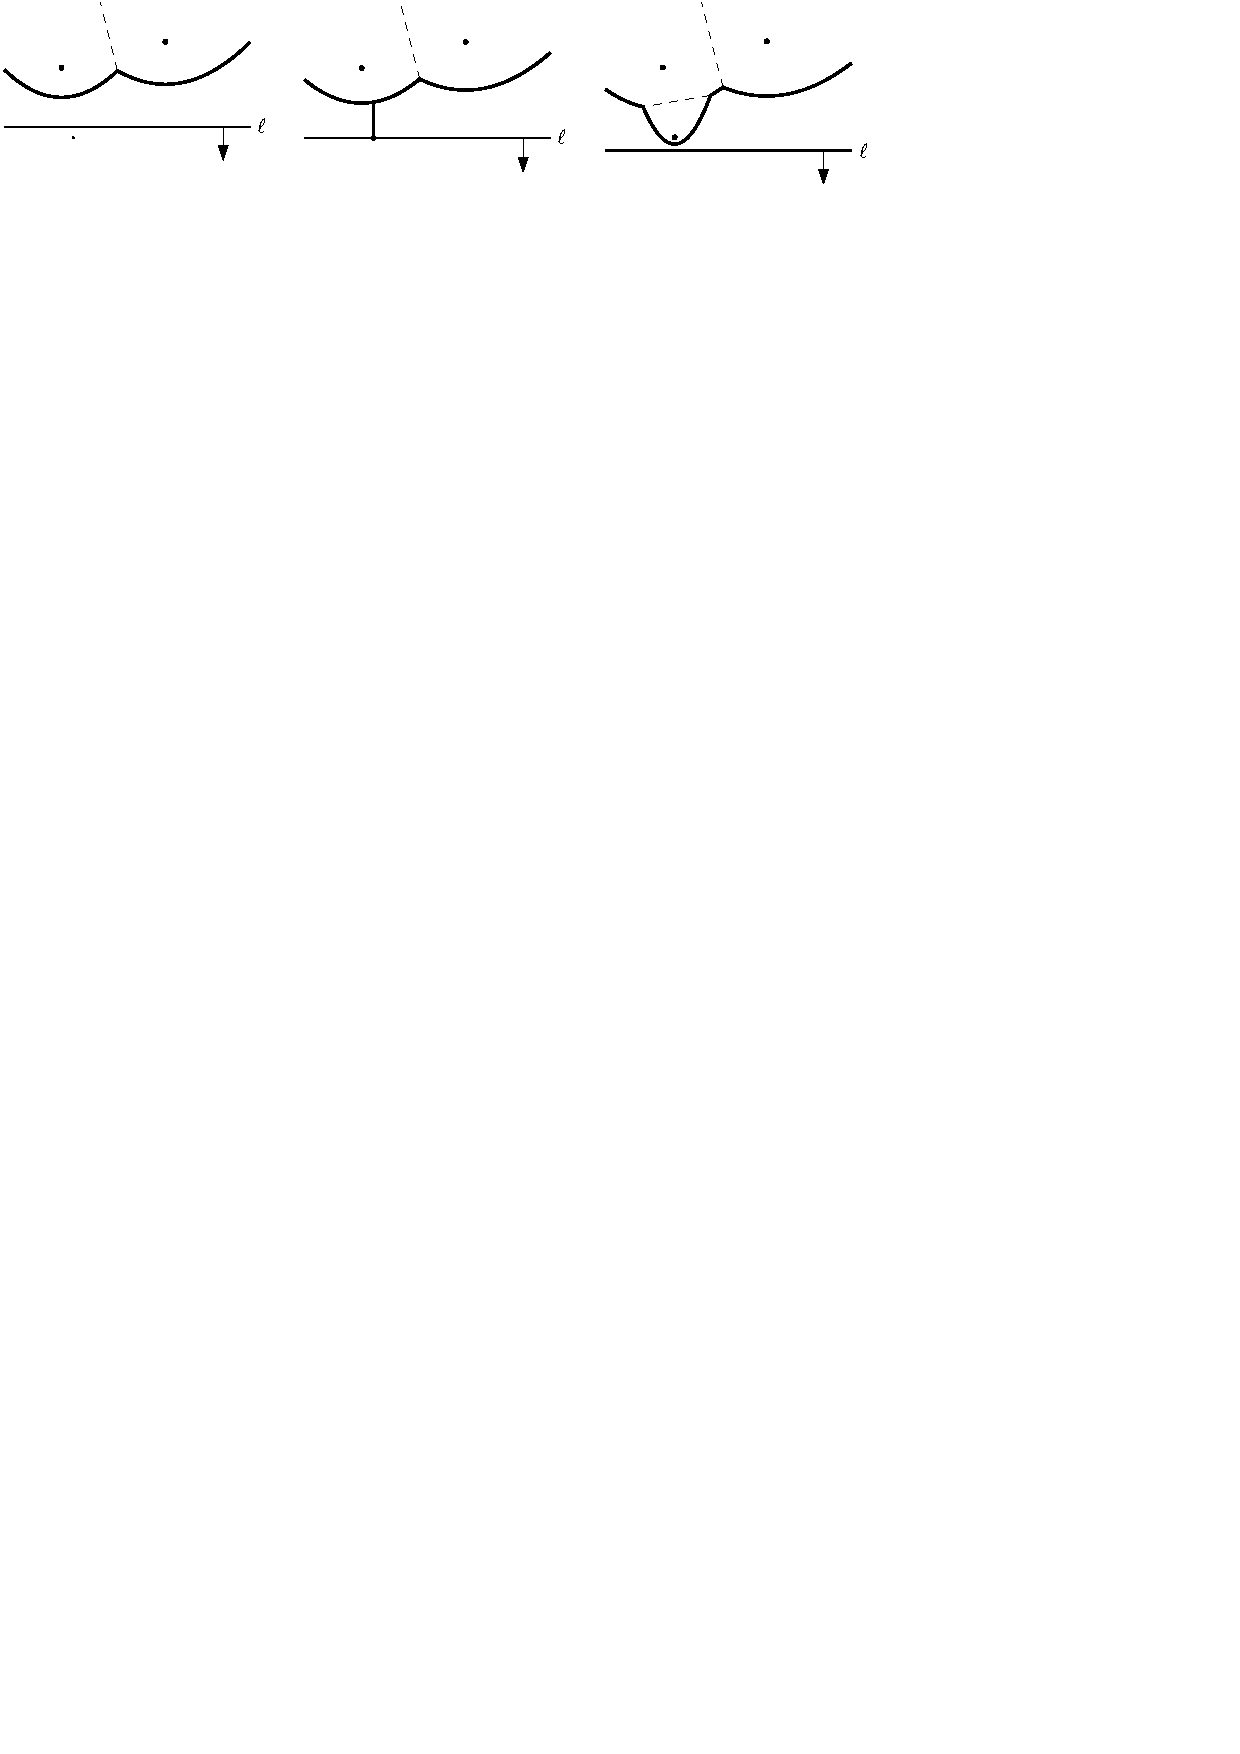
\includegraphics[width=\textwidth]{../images/siteevent}
\]
\pause
Dette kalder vi for en \textit{site begivenhed}.
\end{frame}

\begin{frame}
\pause
Vi så at der bliver fjernet en kurve fra kystlinjen når to Voronoi diagram kanter mødes.
\[
	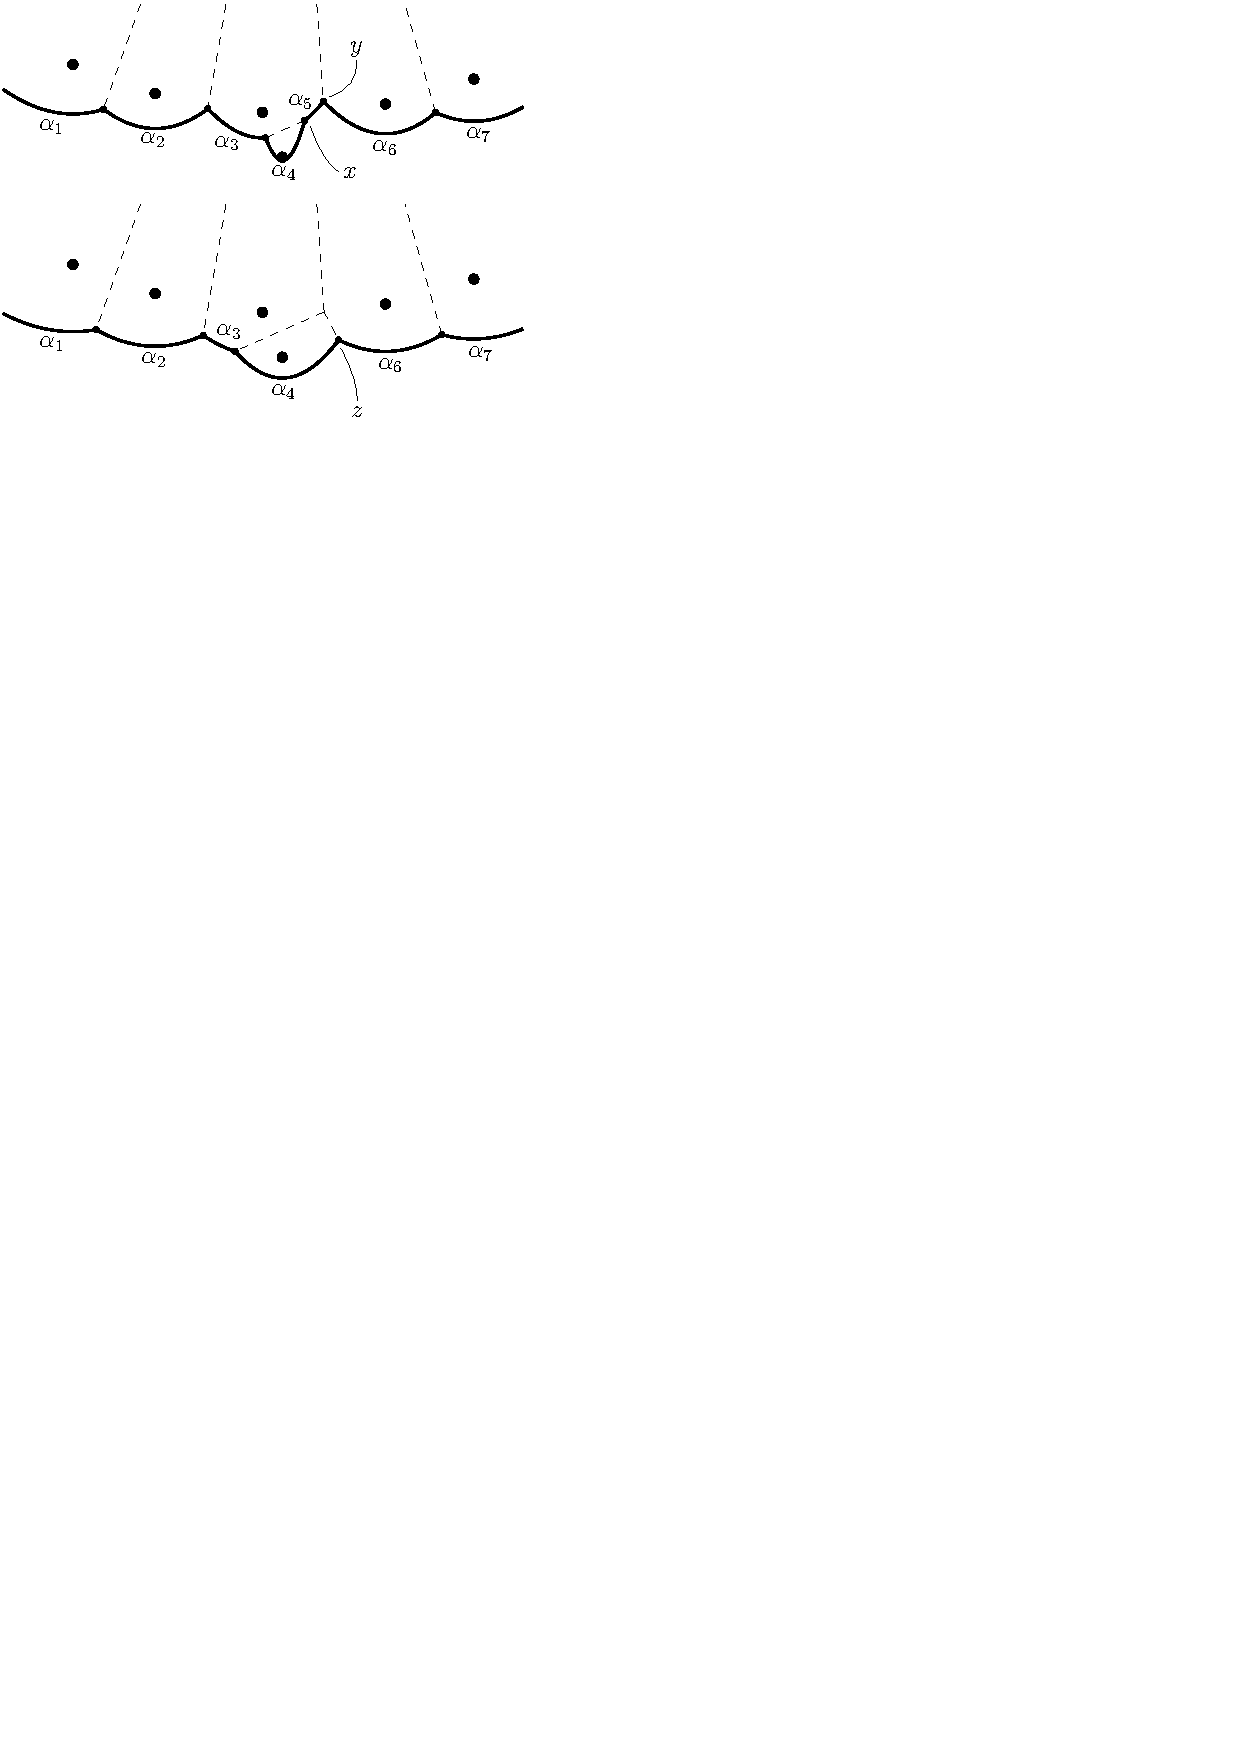
\includegraphics[scale=0.8]{../images/circle_event_beachline_merge}
\]
\pause
Dette kalder vi for en \textit{cirkel begivenhed}.\pause..indtil videre. Det er lidt mere teknisk og kommer senere.
\end{frame}

\begin{frame}
\pause
Ved en site begivenhed begynder en ny kant fra Voronoi diagrammet at vise sig.
\longpause
Ved en cirkel begivenhed bliver to kanter forbundet, og vi får en ny knude for Voronoi diagrammet, og en ny kant fortsættes.
\longpause
Når vores sweep line $\ell$ har været i gennem alle begivenhederne i ordnet rækkefølge opdager vi da hele strukturen på Voronoi diagrammet.
\end{frame}

\begin{frame}
\pause
Vi kommer til at se at for $P$ med $n$ punkter at der kun er $\mathcal{O}(n)$ site og cirkel begivenheder.
\longpause
Vi behøver altså kun at flytte $\ell$ et endeligt antal steder hen, for at opdage strukturen på Voronoi diagrammet.
\longpause
Nu til de tekniske detaljer...
\end{frame}

% % % % % % % % % % % % % % % % 
%
%
% MATEMARISK TEORI
%
%
% % % % % % % % % % % % % % % % 

\begin{frame}
\pause
\[
	\huge\text{Matematisk teori}
\]
\end{frame}

\begin{frame}
%Let \dist(p, q) denote the Euclidean distance between two points p, q \in \R^2.
%    
%This is explicitly given as
%
%    \dist(p, q) = ||p - q||_2, where ||v|| = \/v_1^2 + v_2^2.
%
%Defn (Voronoi cell). Let p_1, p_2, ..., p_n denote the points in P. Then we define the Voronoi cell of the site p_i to be
%
%    V(p_i) = { q \in R^2 | dist(q, p_i) < dist(q, p_j) for all i != j }
%
%<Drawing of a small Voronoi diagram with some V(p_i) marked>

\pause
Lad $\dist(p, q)$ betegne den Euklidiske afstand mellem $p, q \in \R^2$. \pause Dvs.
\[
	\dist(p, q) = \norm{p - q}\pause, \quad \text{hvor} \quad \norm{(x, y)} = \sqrt{x^2 + y^2}.
\]
\pause
\begin{block}{Definition (Voronoi celle)}
\pause
For $p_i \in P$ definerer vi \textit{Voronoi cellen for} $p_i$ \pause til at være
\[
	\mathcal{V}(p_i) = \makeset{q \in \R^2}{\dist(q, p_i) < dist(q, p_j) \text{ for alle } i \neq j}.
\]
\end{block}
\end{frame}

\end{document}